\chapter{Core Systems Design}
\label{cha:core_system_design}
\section{Requirements Analysis}
\subsection{User Requirements}
The following user requirements for the system were gathered by inspecting similar systems, personal creativity and feedback from the supervisor or wearables lab team. User stories were chosen for representation: \ref{table:userStories}.
\begin{center}
        \begin{longtblr}[
            caption={User Stories},
            label={table:userStories}
        ] {
            colspec = {|X|X|},
            rowhead = 1,
            hlines,
        }

        User Story & Acceptance Criteria  \\ 

        As a user I can view health data originating from Oura and Withings devices on a single central dashboard UI so that I can quickly compare measurements between the devices and also manually examine my physical activity and sleep trends.
        & 
        Given that the user is authenticated when the user is on the dashboard page, the dashboard is displayed, containing a graph visualising the last 7 days of data from both devices, with each line coloured differently for each device; also buttons to switch which property, such as steps per day, should be displayed on the graph.
        \\ 

        As a user I can download all of my data as a CSV file by pressing a button in the UI, so that I have my personal data conveniently in one file, in a widely supported format, which could be used for backing up my data to other storage solution, running data analysis etc.
        & 
        Given that the user is authenticated when the user presses the 'Export CSV' button on the main page's UI, the CSV file download starts, with that file containing all of the health measurement data present in the system's database.
        \\ 

        As a user I can critically reflect on the past day, with helpful insights and data presented on the UI; I also want to be reminded about this every day at a certain configurable time; So that I can assess my progress towards my health goals, take pride in my accomplishments today and identify areas to improve on tomorrow.
        & 
        Given that the user is authenticated, at a user-configured time, the user is notified about daily report being available. On the daily report UI page, there is feedback highlighting areas of achievement and areas to improve on; as well as a graph visualising user's progress towards their weekly activity goals, as well as how well/poor the predicted daily activity norm was achieved
        \\

        As a user I can critically reflect on the past week, with helpful insights and data presented on the UI; I also want to be reminded about this every week at a certain configurable time; So that I can assess my consistency in physical activity or sleep, as well as compare this with the previous week.
        &
        Given that the user is authenticated, when the user-configured time is reached, the user is notified about the weekly report being available. On the weekly report UI page, there are graphs visualising consistency in key metrics of MET minutes and sleep score; as well as numerical value quantifying the consistency, with a comparison to the 3 previous weeks. 
       \\

       As a user I want to receive activity reminders throughout the day at configurable times containing a list of curated exercises each with a description and video example on how to perform them, that are well suited to my preferences and health data so far in the week; So that I am encouraged to reach my weekly activity goals; saving time by not having to create a good exercise regiment myself or saving money by not paying somebody else to do it.  
       &
       Given that the user is authenticated, when the user-configured time is reached, the user is notified about daily exercise. On the exercises UI page, there is achieved to expected activity counter and curated list of exercises, which respect the following user-configured preferences: athleticism level, MET weekly target, excluded activities, gym days and home equipment; as well as taking gathered health data into consideration.
       \\
       As a user I can submit free-form natural language questions and then receive natural language answers, which should be influenced as required by my health data and my profile; accessible through UI. So that I can have a natural conversation about my health as I would with a real-life personal trainer, providing guidance and a sense of not being alone.
       &
       Given that the user is authenticated, when the user visits the AI Chat UI page there is a chat containing past user's requests and system's responses; there is an input box where the user can type a question using natural language. After submitting the question a reply is sent, which takes into account the user's health data and their profile.

        \end{longtblr}
    \end{center}

\subsection{Functional Requirements}
The following functional requirements were derived so that user requirements could be fulfilled. System use case diagrams, flowchart and textual descriptions were used as representations.
\begin{itemize}
    \item Sync and view data diagram: \ref{fig:2}
    \item Export data diagram: \ref{fig:3}
    \item Daily \& Weekly Reports diagram: \ref{fig:4}
    \item AI Inference flowchart: \ref{fig:5}
    \item Activity Plan diagram: \ref{fig:6}
    % \item Personalisation: User is able to configure their profile, which is saved in the database and used to customise modifiable parameters of the system. The profile has the following fields: 
    % \begin{itemize}
    %     \item Height in cm: Integer
    %     \item Weight in kg: Integer
    %     \item MET minutes weekly target: Integer
    %     \item Excluded activities keywords List of strings
    %     \item Athleticism: Enum [Beginner, Intermediate, Expert]
    %     \item Gym days: List of Days of the week
    %     \item Home equipment: List of strings
    %     \item Report notification time: Time
    %     \item Daily activity reminder times: List of times
    % \end{itemize}
\end{itemize}
\begin{figure}
    
    \centering
    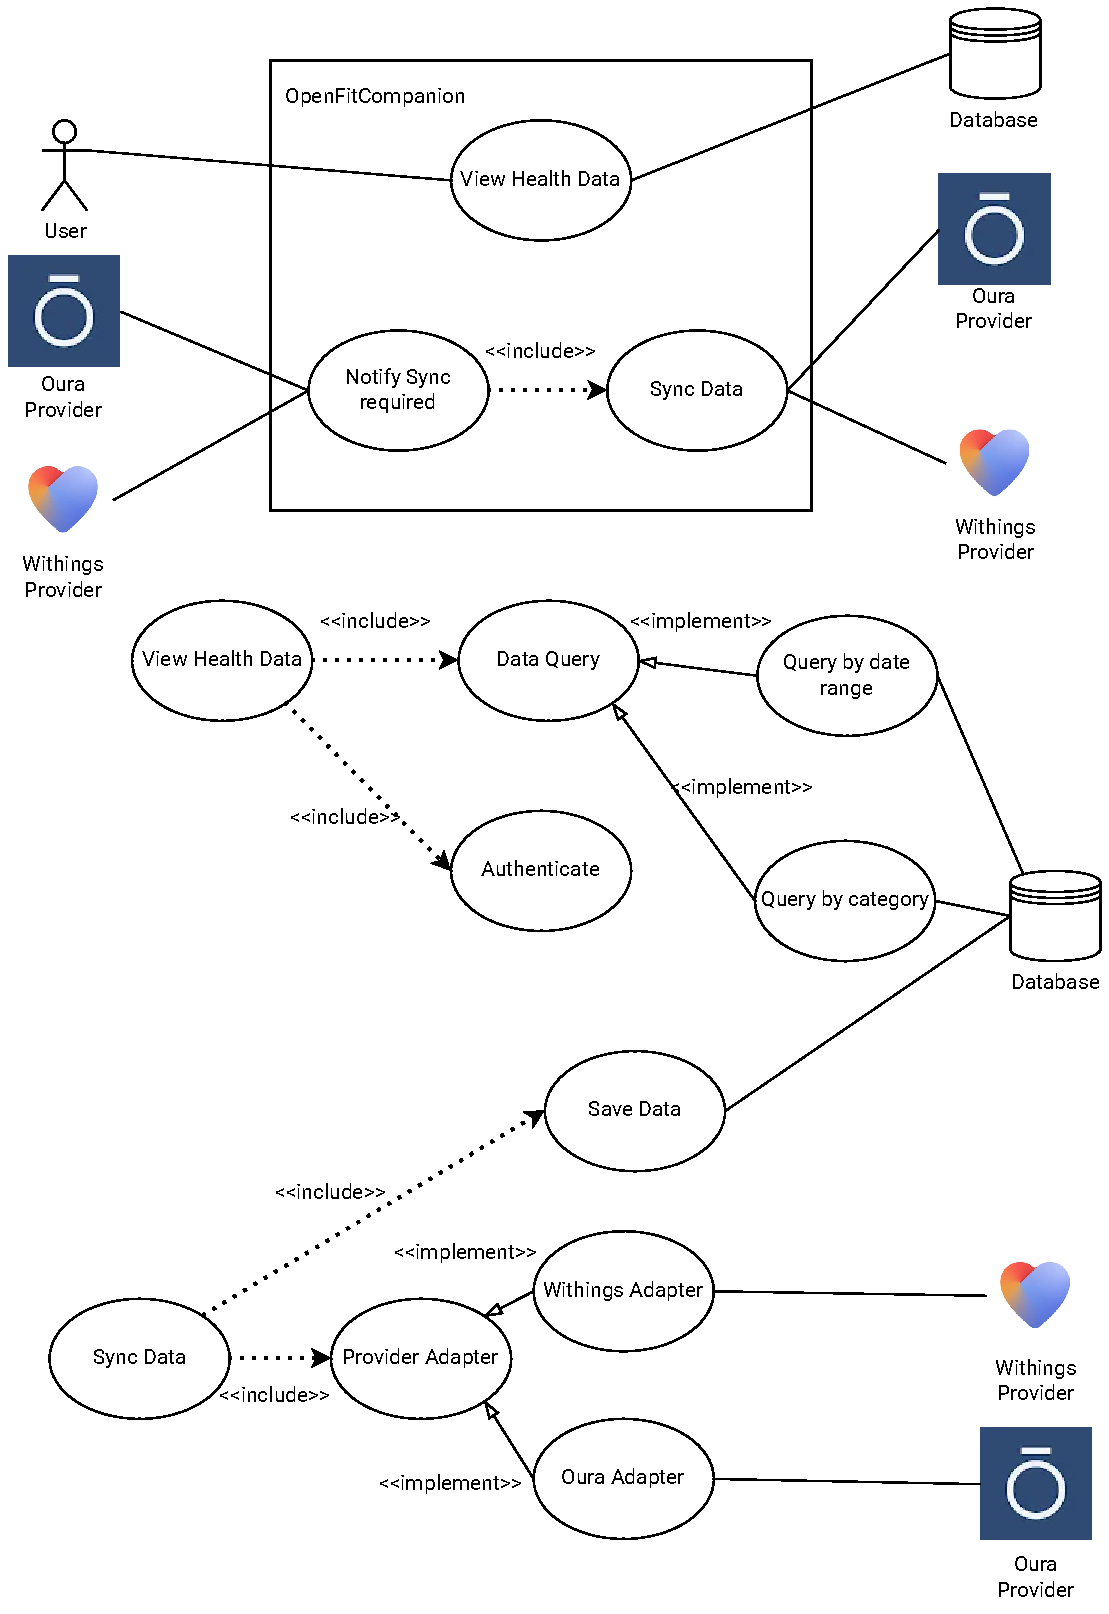
\includegraphics[width=0.9\textwidth,keepaspectratio]{../images/viewFunc.pdf}
    \caption{View data use case UML diagram}
    \label{fig:2}
\end{figure}
\begin{figure}
    
    \centering
    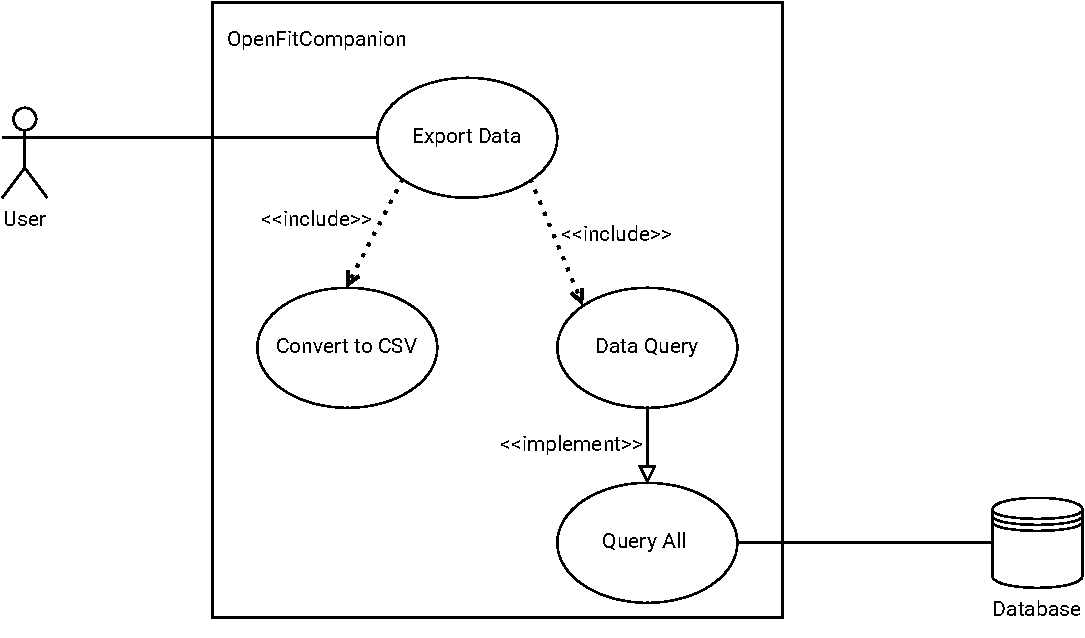
\includegraphics[width=\textwidth,keepaspectratio]{../images/exportDataFunc.pdf}
    \caption{Export data use case UML diagram}
    \label{fig:3}
    
\end{figure}
\begin{figure}
    
    \centering
    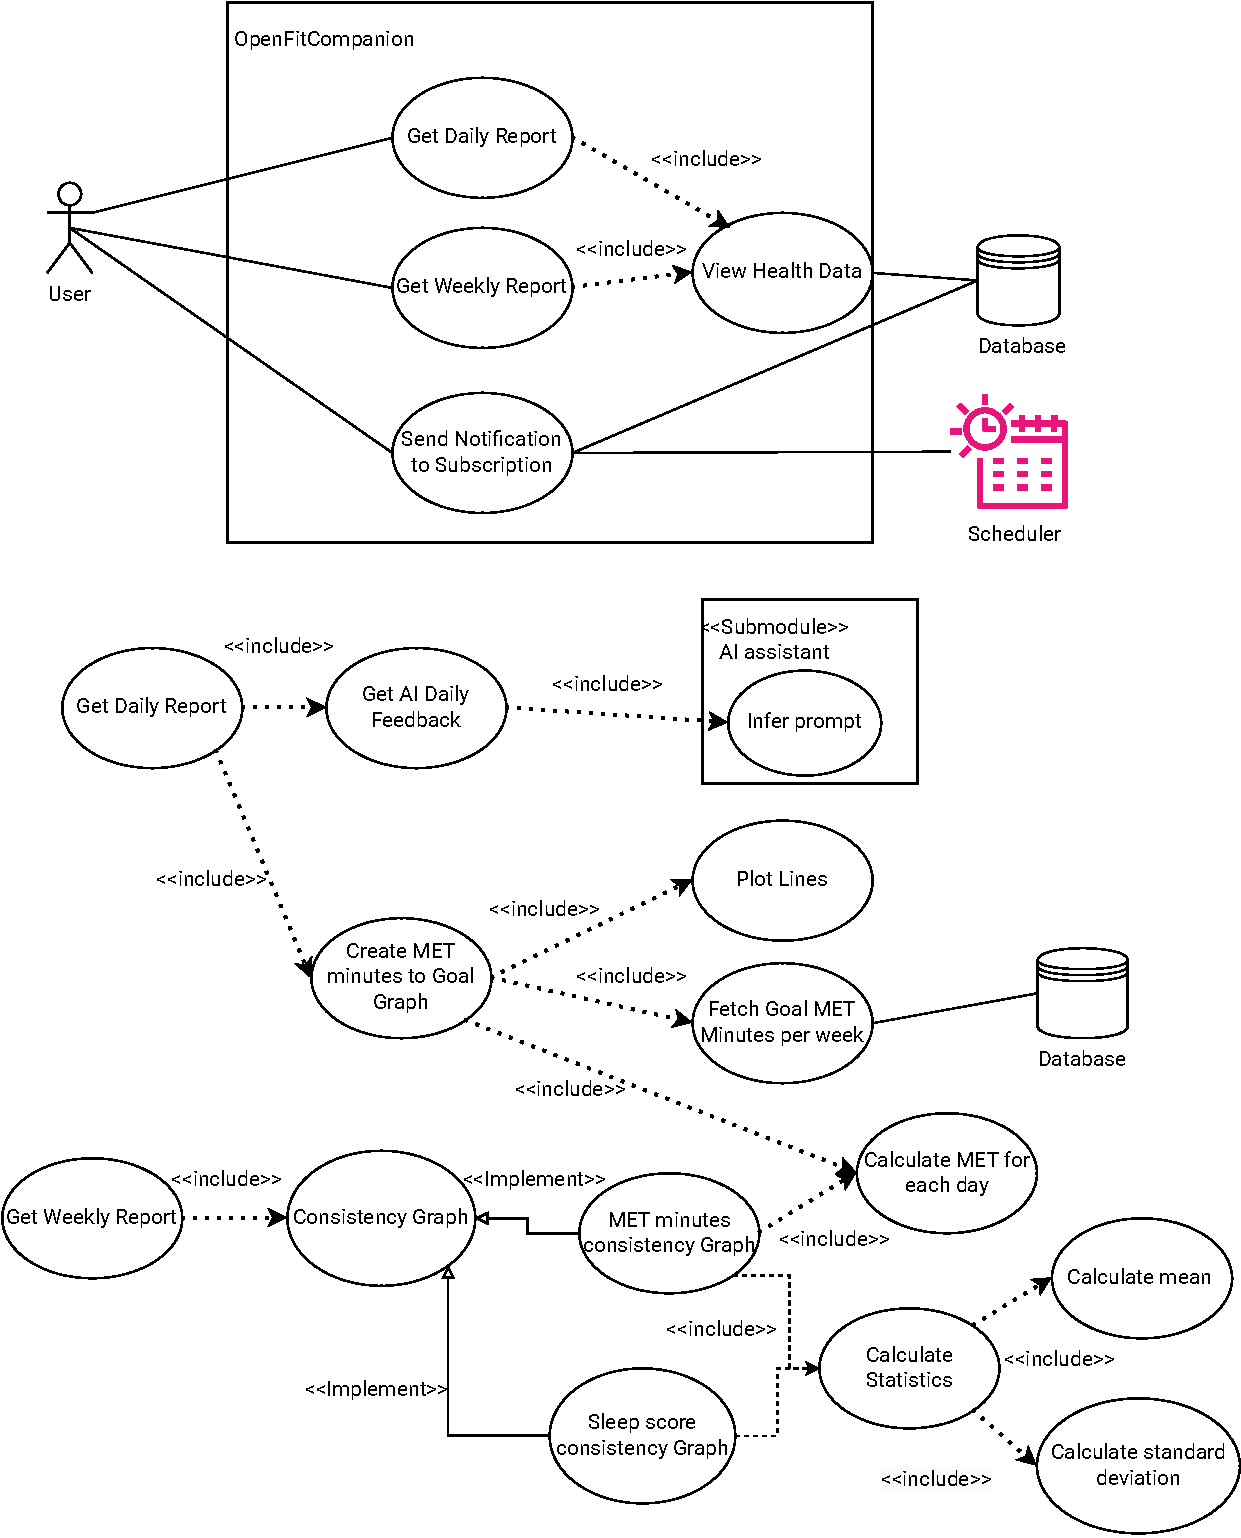
\includegraphics[width=\textwidth,keepaspectratio]{../images/reports.pdf}
    \caption{Daily \& Weekly Reports use case UML diagram}
    \label{fig:4}
    
\end{figure}
\begin{figure}
    
    \centering
    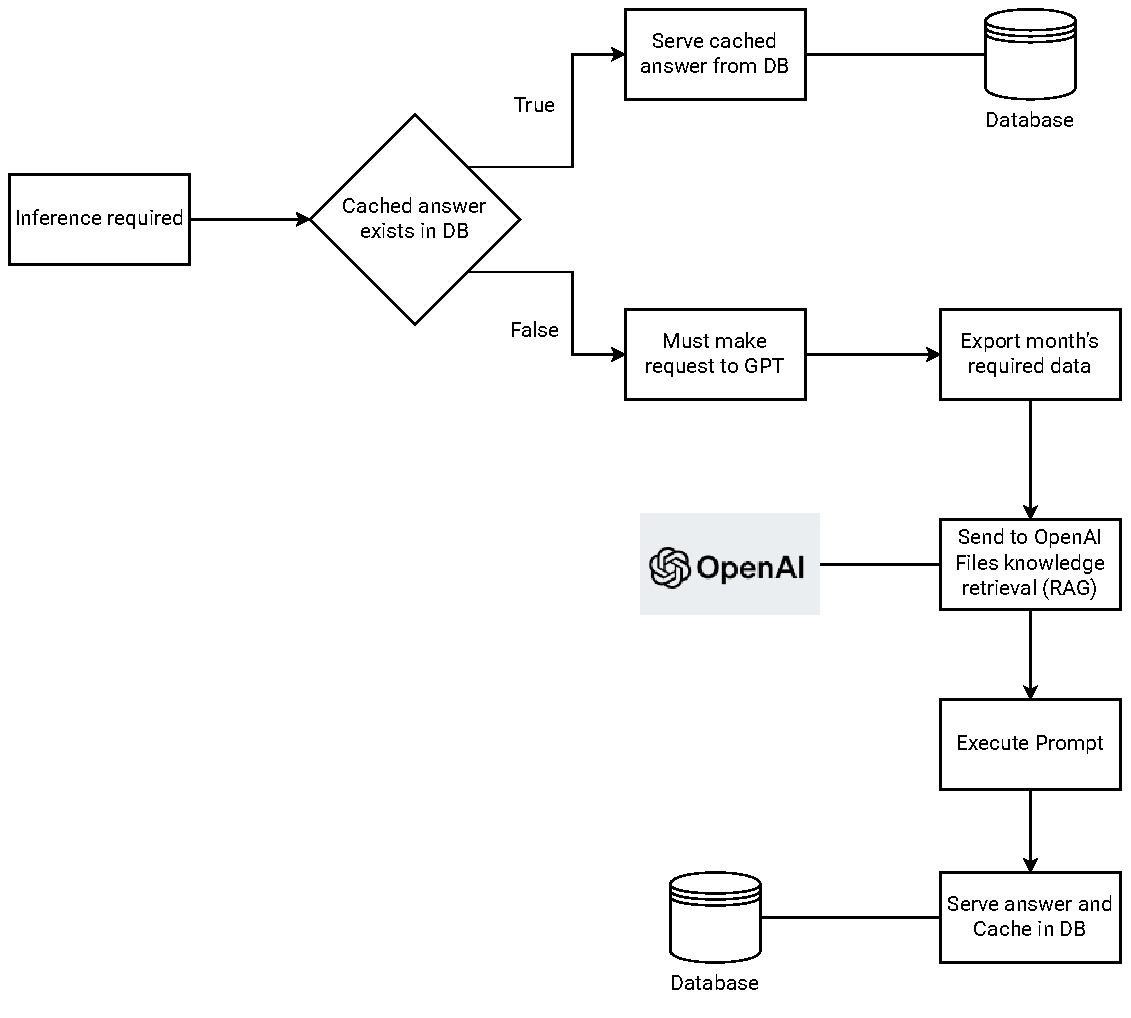
\includegraphics[width=0.95\textwidth,keepaspectratio]{../images/ai.pdf}
    \caption{AI Inference functionality Flow Chart}
    \label{fig:5}
    
\end{figure}


\begin{figure}
    
    \centering
    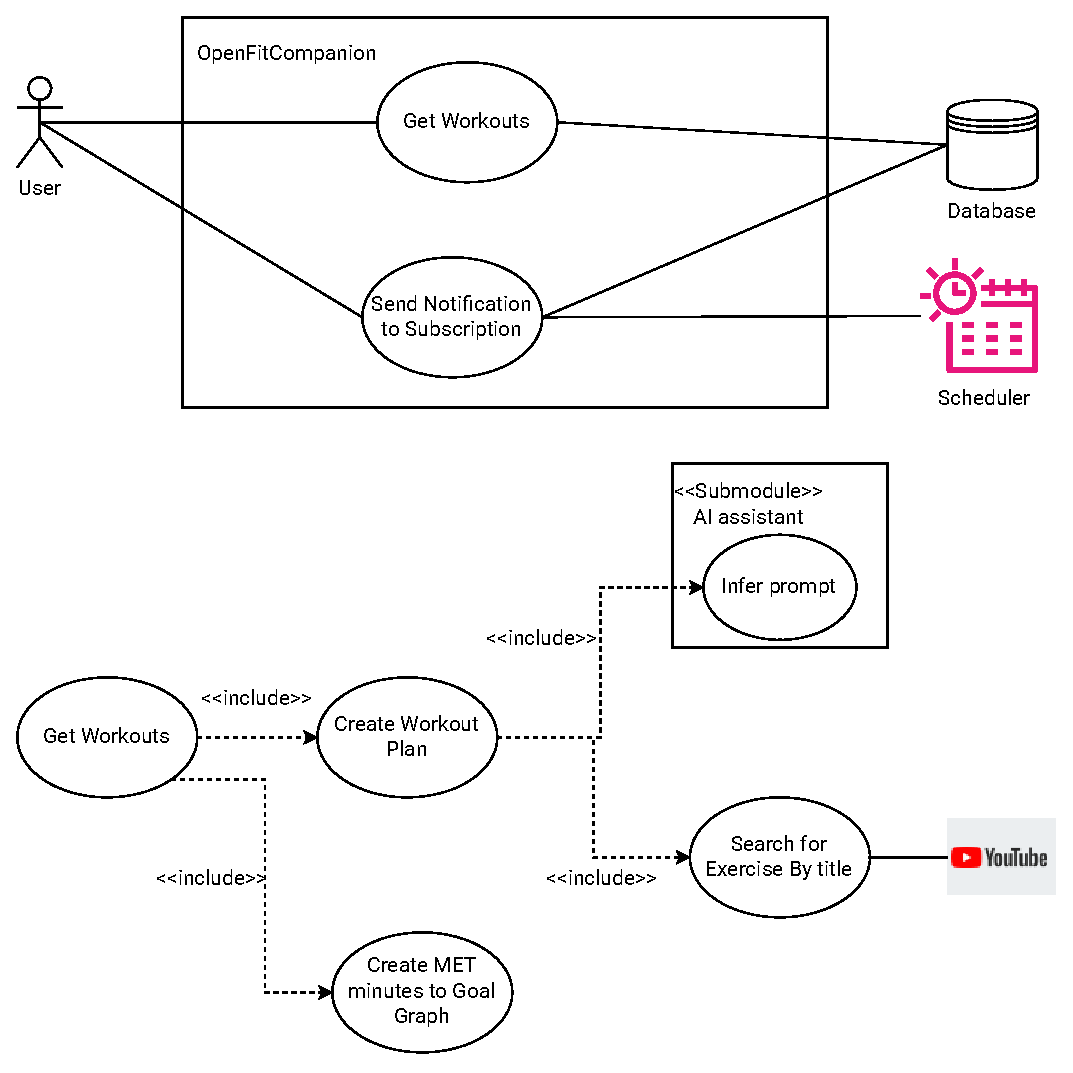
\includegraphics[width=\textwidth,keepaspectratio]{../images/workouts.pdf}
    \caption{Activity plan use case UML diagram}
    \label{fig:6}
    
\end{figure}
\subsection{Non-Functional Requirements}
The following non-functional requirements for the system were gathered by inspecting general best practices and common sense. Represented as textual descriptions. 
\begin{itemize}
    \item Security: System must be secure and only allow access to the authenticated user. 
    \item Performance: UI must have low latency and feel snappy when used on a mobile network. 
    \item Usability: UI must be comfortably usable on mobile, openable as a native mobile app and support push notifications in the background (even if the app is closed).
    \item Accessibility: UI must follow best practices supporting usage with assistive technologies such as screen readers, keyboard only etc.
    \item Extensibility: The whole system should be easy to maintain and add new features, feature comprehensive logging and scalability to add more providers.
    \item Cost: Cost of running the service should be minimised while retaining the required functionality.
\end{itemize}
\section{High-level overview}
\begin{figure}
    
    \centering
    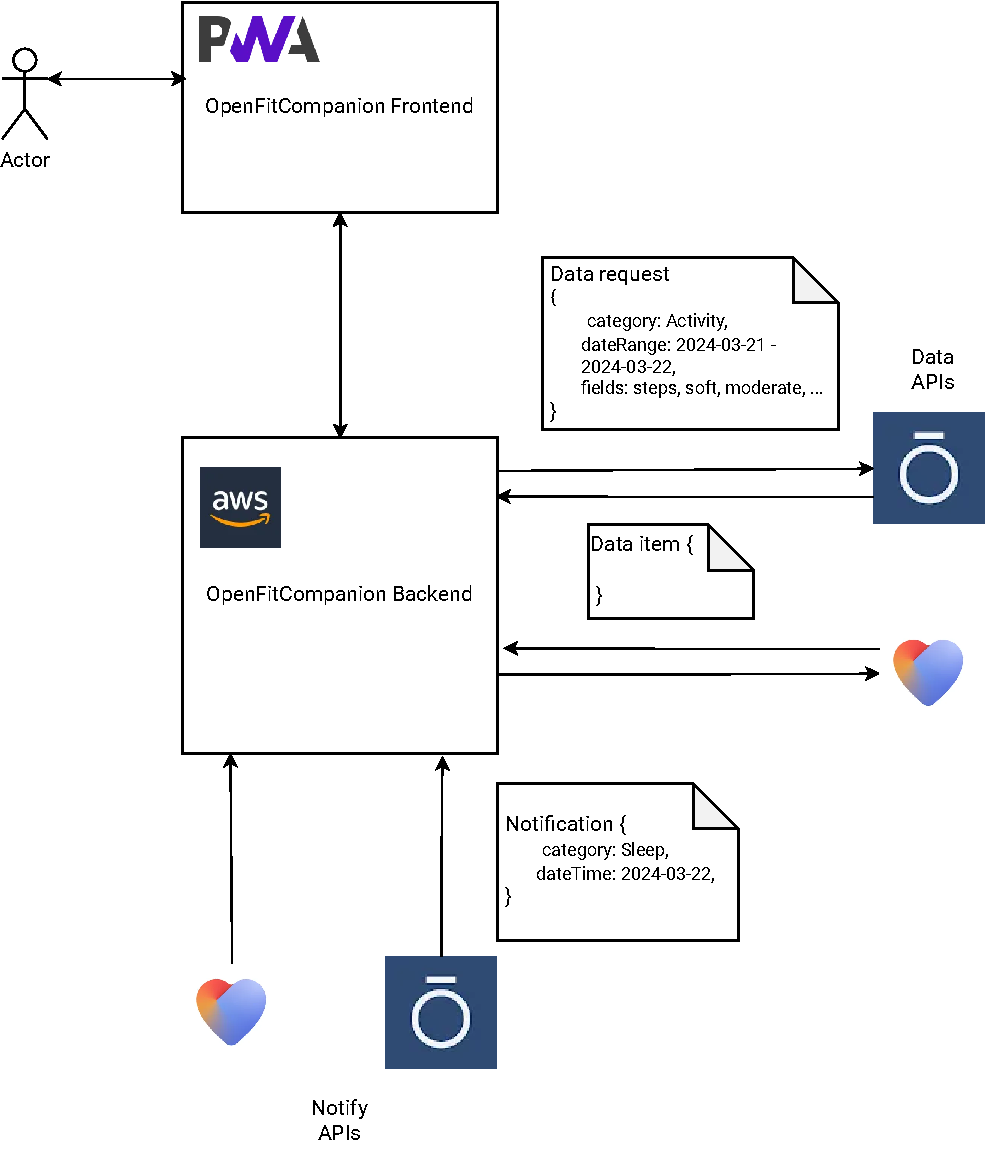
\includegraphics[width=0.95\textwidth,keepaspectratio]{../images/highLevel.pdf}
    \caption{High-Level architecture diagram}
    \label{fig:1}
    
\end{figure}
Overall, the architecture is structured as a composition of event-driven microservices. Computation only needs to happen in response to an external event. This is enabled by providers supplying Webhook integrations. Essentially, the backend gets a notification from providers whenever there is new data available from them. The microservices approach allows for much stronger fault tolerance, whereby a fault in one part, does not bring the entire service down; for example, a bug in interfacing with the providers won't prevent the user from accessing the UI and the associated API endpoint with the database. It is also far cheaper than a monolithic service. The following is the diagram together with sample data exchanged: \ref{fig:1}

Cloud-deployed backend service receives notifications from providers, containing information that allows atomic processing of that notification. 

In response to the notification, the backend sends a request to the Data APIs of providers, receiving an item(s) back and finally persisting it in a database for further purposes. 

Withings and Oura providers were integrated at the time of this report. However, the system can scale to many more providers. The only requirement for a provider is that they have Data API we can use. Even if a particular provider did not have a webhook (notification) service, we could re-sync with data APIs on a regular schedule, like every 30 minutes. With the interval value being a trade-off between potentially more latency in syncing the data or wasted compute time when there are no updates. This would be quite costly if the system was a publicly available service, as that scheduled request would be needed for each user. However, for our use case of self-deployed service, the cost is negligible. However, there is still a reliance on provider's API services to get the actual data from devices. The system does not communicate with the smart devices directly via Bluetooth, there is an intermediate provider's system that data must pass through. So, if a provider does not have such a service, we can't integrate them.

Ultimately, the data is transformed into useful information (insight) using LLMs and classical algorithms. This is then presented to the user through the frontend. 
\begin{itemize}
    \item {Dashboard, contains a graph visualizing data from all devices, allowing for comparison and a brief overview of trends.}
    \item {Daily Report, containing a graph visualizing MET minutes completed this week and the goal MET minutes per week; Feedback on expected activity completion for that day and AI feedback for that day. Provides the user with information, allowing them to reflect on their day and see the progress towards fulfilling the weekly activity goal. A notification is sent to the user when such report is available. This constitutes a Type 2 nudge, as it engages the user's conscious, reflective thinking to get them more motivated for physical activity tomorrow. However, there is also a component of Type 1 nudge with report notifications being opt-out rather than opt-in.}
    \item {Weekly Report, focusing more on consistency rather than absolute values and goal completions. Contains a graph visualizing deviation from the mean value of daily activity or sleep score. Same nudging as Daily Report.}
    \item {Activity plan, containing a curated list of planned physical activities for the day, generated by AI. Also containing feedback about activity minutes done today. Similarly, it has a Type 1 nudging factor, being opt-out as well as Type 2 nudging, by notifying users at certain times when they should be doing exercises, and providing a well-suited list of exercises, with description of benefits and video examples on how to perform them. This removes the need for user to plan their own workouts, removing decision paralysis. Also imitates real-life coaching with a personal trainer, bringing benefits such as accountability and personalisation.}
\end{itemize}

\section{Back-end}


\subsection{Compute}
Serverless functions are used as the main computing units for the backend. For AWS that is Lambda. Using Lambda is the most cost-effective option; it allows paying only for execution time down to milliseconds, and free data-out transfer to other AWS services. Also, there is no need to configure and manage servers. One disadvantage is cold starts, when a function is called for the first time in a while, it has increased latency due to some set-up, from experiments, it's around 400ms on average. That happens for all Lambda functions, so if there is a chain of such functions called one after another, the latency will stack up and be quite noticeable. AWS provides the "Provisioned Concurrency", making sure that N functions are kept initialised and ready to respond at any time, however, it has a separate costing scheme similar to servers, whereby you pay by the second even if the function is never called. As per project aims, minimising cost is important so the latency is something that is just tolerated. All configurations are set to the lowest costing option, such as using an ARM processor, 128Mb RAM and 512Mb Storage.
\subsection{Technologies}
Typescript running on NodeJS was the chosen programming language. NodeJS has a very easy-to-use asynchronous programming model, which is preferable in this use case, as most tasks are I/O bound; so that many other tasks can be executed in parallel, such as fetching multiple rows from the database. Typescript provides static type safety, which helps to avoid bugs in an otherwise type unsafe JavaScript, as well as better developer experience with enhanced auto-completion in a modern IDE. This increases the speed of development and makes the project more attractive to potential open-source contributors.
\subsection{Persistence}
For persistence, DynamoDB is used. It is well integrated with AWS infrastructure, has low latency, schemaless and low price which is covered by Free Tier. Because the service is meant to be used by a single user who is the owner of the self-deployed infrastructure, there is no need to identify to which user the row of data belongs. Since DynamoDB, like most NoSQL databases does not support composite keys i.e. keys that are made from 2+ fields; meaning that complexity has to be handled client-side. For example, using field1 and field2 as PK involves having single field PK and using something like "field1\_\_DELIM\_\_field2" as the value, and checking that delimiting string does not form naturally (which is unlikely) from field values to ensure uniqueness. To improve robustness a simple client-side schema that relies on Typescript classes was designed. Primary key schema is derived by considering access patterns to that table. For example, with health data: \ref{fig:schema}, the typical functionality is querying a certain data type (sleep, activity) originating from a certain provider between a range of dates; using the key schema in the diagram, this typical request can be handled efficiently by setting composite partition key and using DynamoDB range query of BETWEEN with no need for expensive client-side filtering. Provisioned capacity (does not scale with demand) mode is used, with the number of read and write units set to 1. This minimises the cost but increases latency due to restricting parallelism to 1 access at a time, but it is largely unnoticeable as DynamoDB inherently has a very low latency. AWS automatic encryption of data at rest is used, which incurs no charge, ensuring that even if the database is leaked, it can't be accessed and vulnerable health data is protected.
\subsection{Miscellaneous}
All of the AWS services are deployed on AWS us-east-1, which is in the US, state Virginia on the East Coast. This particular deployment region was chosen because some services, such as DynamoDB cost more in Europe, and the east of the US is closer geographically to the UK, minimising network latency. AWS IAM roles for each service were created according to the principle of least privilege, ensuring that each service only has access to the infrastructure it requires to function and not more - minimising attack surfaces and malware propogation capabilities.
\begin{figure}
    
    \centering
    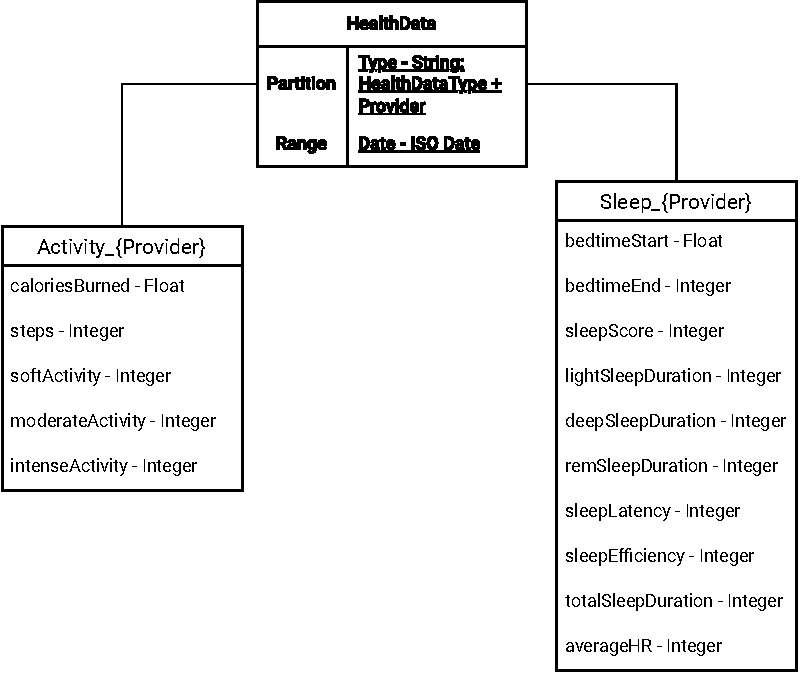
\includegraphics[width=0.9\textwidth,height=\textheight,keepaspectratio]{../images/dataSchema.pdf}
    \caption{HealthData Table client-side Schema}
    \label{fig:schema}
    
\end{figure}
\subsection{Unifying}
Although data from all devices is stored and can be viewed separately, for many purposes such as AI insights there needs to be a single row for each day that is treated as the ground truth. For this, measurements from all devices are averaged out and stored under the "Unified" Provider. 
\subsection{Architecture}
\begin{figure}
    
    \centering
    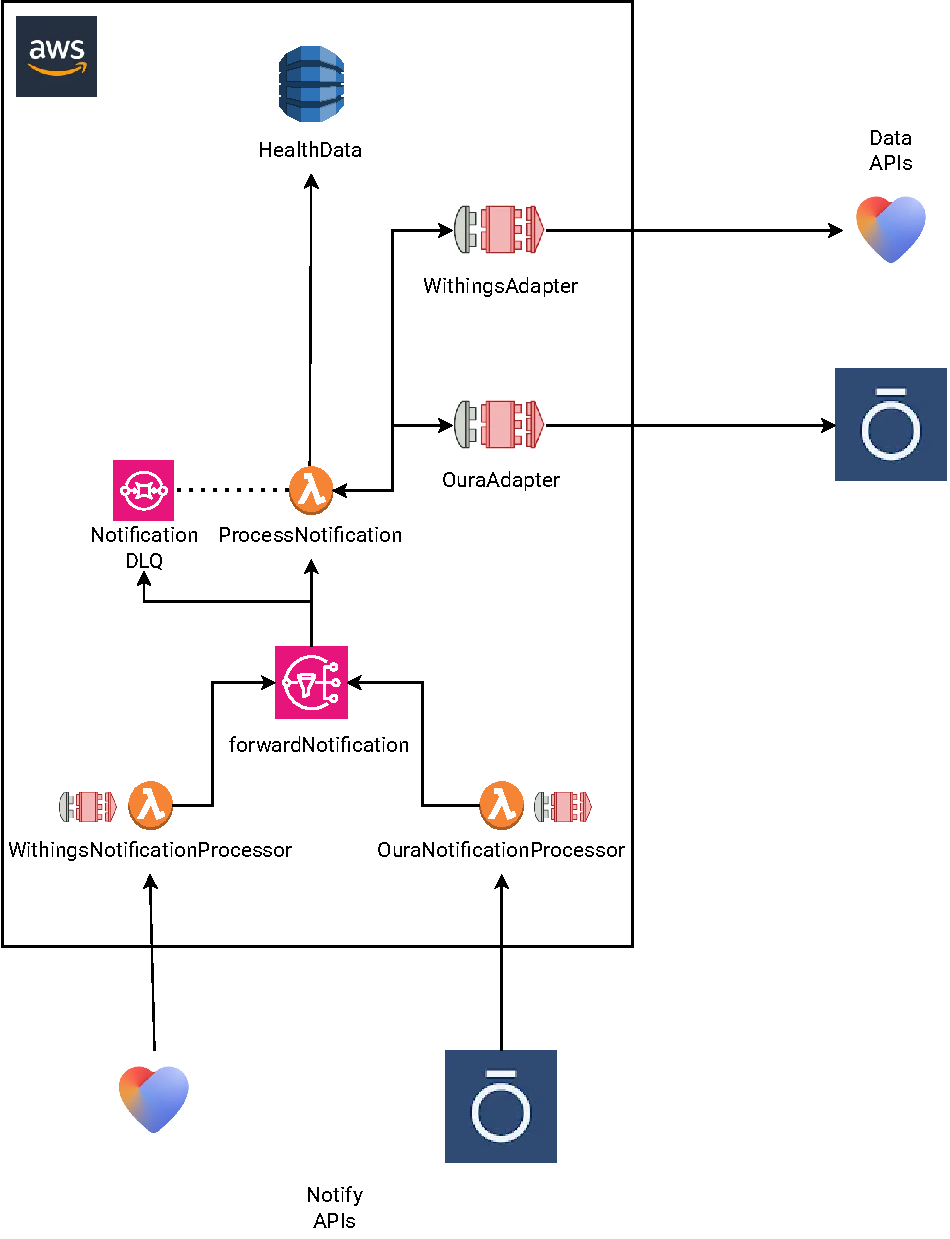
\includegraphics[width=0.95\textwidth,height=\textheight,keepaspectratio]{../images/backend.pdf}
    \caption{Back-end Architecture Diagram}
    \label{fig:backend}
    
\end{figure}
Breaking down the purpose of each component in \ref{fig:backend}: (Note: Some of the backend components will be presented in the next section)
\begin{itemize}
    \item {WithingsAdapter \& OuraAdapter: Software classes for abstracting complexities of interfacing with external providers - Adapter pattern. Different providers require different: formats for the request, authentication, attribute unit conversions, etc. These adapters handle such intricacies while providing an easy, consistent interface.}
    \item {WithingsNotificationProcessor \& OuraNotificationProcessor Lambdas: Handles webhook notification HTTP requests, extracting relevant information and passing it to the SNS. There are 2 of them because notifications from different providers require different processing. Uses adapter components for handling this different processing.}
    \item {ForwardNotification SNS \& NotificationDLQ: Decouples the system, as Lambdas directly invoking other Lambdas is a bad practice: worse observability, harder exception handling, etc. SNS is preferable to queue because it fits in a serverless architecture better and costs less due to it being a push model rather than queue polling. Failed requests from SNS are sent to the Dead-Letter-Queue (DLQ), where they are saved so that they can be re-processed later; this allows the system to tolerate external service faults.}
    \item {ProcessNotifcation Lambda: Triggered by notification, uses adapters to request data item(s) from providers and stores it in the database. For example, Withings uses OAUTH, with authentication tokens alive for 4 hours; if required, refresh the authentication token before doing the request. Performs a manual poll of DLQ, executes any notifications that are in the queue. A manual poll is preferred because it does not cost nearly as much as automatic polling of the DLQ, however, the disadvantage is the increased latency, as failed notifications from DLQ will only be re-tried on the next normal notification received. }
\end{itemize}
Integrating more providers comes down to only writing adapter implementation for them, the rest of the architecture stays the same. This makes the system easily extendable to any number or kind of providers.
\section{Front-end}
\subsection{UI}
For the user-facing application, the eight golden rules of interface design \cite{goldenRulesUI} were followed when applicable, as well as striving to be minimalistic and only including relevant info.
\subsection{Technologies}
The application is a Progressive Web App (PWA) implemented using React, Typescript and other application-specific libraries. PWA allowed the application to be installable and used as a native app on many devices including PC, android, and iOS. Offering native functionalities such as background push notifications, while built as a website using standard platform-agnostic technologies; this enhances maintainability, as there is no need to maintain multiple versions for different platforms. Also, web development is more widespread than native app development, allowing more people to potentially contribute to the project. Similarly to the backend, Typescript offers static type safety which enhances maintainability. React allows writing UI components in a readable, declarative style, without worrying about efficient low-level implementations. Also promoting great code reusability through components, which improves readability by decreasing the number of lines of code. A number of other smaller libraries were used to not re-invent the wheel for the needed functionality, and instead use well-tested and well-documented libraries. For example, Chart.js was used extensively for creating graphs that were modern-looking, easy to use and performant. 
\subsection{Architecture}

\begin{figure}
    
    \centering
    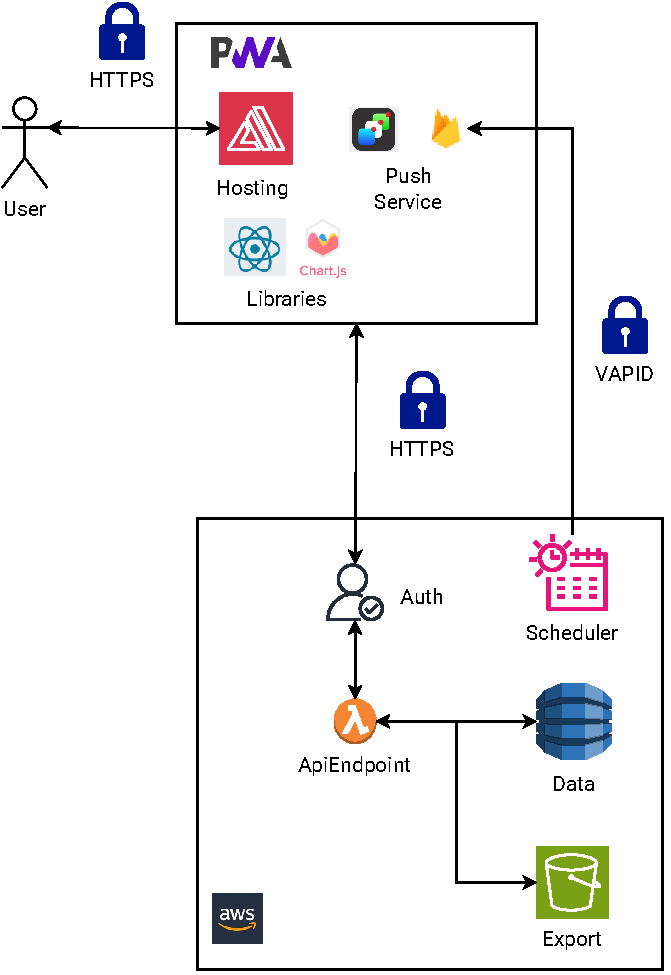
\includegraphics[width=0.7\textwidth,keepaspectratio]{../images/frontend.pdf}
    \caption{Front-end Architecture Diagram}
    \label{fig:frontend}
    
\end{figure}
Breaking down the purpose of each component in \ref{fig:frontend}:
\begin{itemize}
    \item {Authentication: The website is using HTTPS, meaning that all of the contents are securely encrypted. The website is deployed on the internet and authentication is done via a simple secret key. At set-up, the backend generates a random 256-character string containing a diverse set of capitalized characters, numbers and special symbols; it is then configured to only accept requests if the authorization header contains this secret key. The user needs to set the same key in the frontend.}
    \item {Push-Notifications: Push subscription is registered with the browser's push service and sent to the backend. Now, the backend can proactively send notifications to the user using the standard protocol - WebPush, authenticated using VAPID. This is done on a regular schedule which is handled by the AWS EventBridge Scheduler. }
    \item {Hosting: The website is hosted using AWS Amplify. It allows configuring the CI/CD pipeline which consists of creating an optimised site build on every push to the release GitHub branch. File compression (Gzip) is turned on, minimising network transfer time. }
    \item {Export: Firstly, On the backend, All rows of the healthData table are fetched page by page, since DynamoDB restricts a single request to a maximum of 1MB. Then JSON data is converted into CSV using a library and the file is uploaded to an AWS S3 bucket and a one-time download URL is created. Item is deleted from S3 after download. S3 is used instead of directly returning binary blob from Lambda, because there is a 6MB maximum restriction set on Lambda's response body, whereas S3 does not have any file size restriction. }
\end{itemize}
\section{AI}
\subsection{RAG}
GPT4 was used to derive insights and various prompt engineering techniques were applied to enhance the quality. Initially, it was planned to send the health data directly as text in the context window of a generation request. However, even if all relevant health data was included in the context, sometimes the reply contained phrases like: "I don't have the ability to access or review past interactions within this thread or recall personal data unless it's provided again within the current request". The important detail is that it happened sometimes, not all of the time; therefore I suspect this is an example of hallucinations LLMs can experience. A solution that worked was to use the experimental feature - Knowledge Retrieval (RAG). This fixed the missing information hallucination. In theory, only the relevant rows should be sent, so if the prompt was: "use last 7 days to...", then it should only consume tokens for including last week's data; this isn't what happened in practice, for unknown reasons.  Unfortunately, there is a standing charge of 0.2\$ per day, which added to the fact that GPT4 is generally expensive, adds up to quite a high sum. A more detailed cost breakdown is in the evaluation \ref{cha:evaluation}. Overall, the process of using GPT4 is as in \ref{fig:5} with a slight modification. Instead of including data in context explicitly, last month's data is exported into a JSON file and uploaded to OpenAI's files, which is then used by RAG. If able to, a cached copy is served instead of re-generating a response again.
\begin{figure}
    
    \centering
    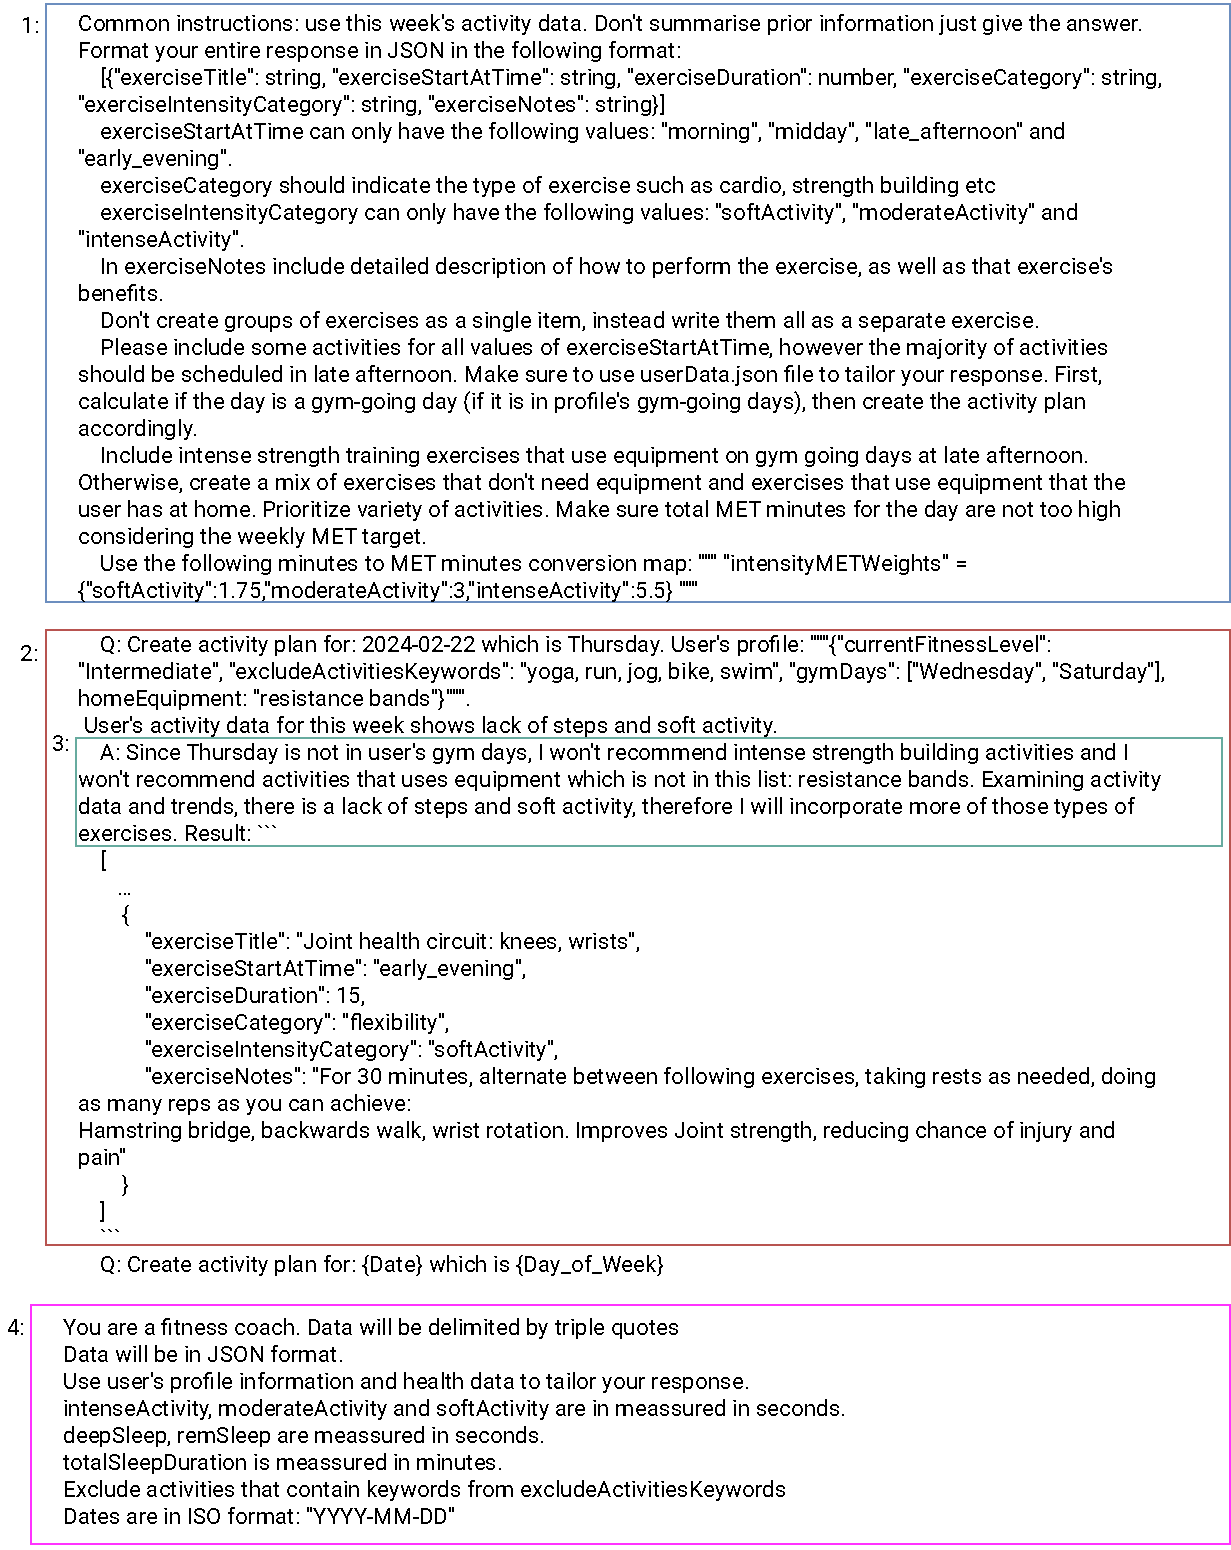
\includegraphics[width=\textwidth,height=\textheight,keepaspectratio]{../images/AIPrompt.pdf}
    \caption{LLM Prompt for activity plan}
    \label{fig:prompt}
    
\end{figure}
\subsection{Prompt Engineering}
Breaking down a prompt used for generating activity plan \ref{fig:prompt}:
\begin{itemize}
    \item 1: Not any technique in particular, simply adding details relevant to the prompt: rules, reply format, etc as much as possible, to guide the model and remove any ambiguity. For example, the "majority of activities should be scheduled in late afternoon" ensures that the activity plan fits a typical schedule of a person since most people will get off work in late afternoon.
    \item 2: Few-shot prompting: in this case, it is a 1-shot prompt. However, it is not a pure application of technique, as the health data in the example is summarised instead of given in full like a true prompt will have. Pure application would not be as effective, because it seems context from RAG is given more priority which can't be replicated manually, and this saves prompt tokens. Through trial and error, using more examples than 1 shown to lead to replies being less creative,  mimicking the examples and not introducing any other novel exercises - overfitting. This noticeably improves the reply quality, without it, sometimes it would recommend exercises that use equipment not owned, suggesting gym exercises on a non-gym day, etc.
    \item 3: Chain of Thought: highlighting the relevant bits from the context and how they affect the response: "Examining activity data and trends, there is a lack of steps and soft activity, therefore I will incorporate more of those types of exercise". Experimentally, the simplistic few-show-CoT is slightly better than zero-shot-CoT. However, zero-shot-CoT is used for monthly feedback prompts, as it would be hard to provide useful examples there.
    \item 4: System Prompt, Role assumption. The system prompt is concatenated to every prompt. The data format units are specified, as well as the LLM's role - a fitness coach. This noticeably improves response quality. For example, since the units are established - totalSleepDuration is in minutes, it can then compare those measurements with the WHO recommendation of 7-9 hours of sleep; the role makes the AI more helpful, understanding that the purpose of the interaction is to help improve the client's health. It also includes more realistic practical considerations, such as suggesting improving sleep schedule by gradually going to bed earlier, instead of just stating scientific best practices.
\end{itemize}